\documentclass[10pt]{article}
\usepackage[letterpaper,top=0.75in,bottom=0.75in,left=0.75in,right=0.75in]{geometry}
%\usepackage{geometry}
\usepackage{graphicx}
\usepackage{amssymb}
\usepackage{amsmath}
\usepackage{enumerate}
\usepackage{float}
\setlength\parindent{0pt}

\title{
\vspace{-20.mm}
Privacy Preserving Biometrics based Remote Authentication Protocol for Mobile Devices}
\date{}
\vspace{-20.mm}

\begin{document}
\maketitle
\section{Motivation:}
There has been a major shift from traditional passwords based authentication to biometrics based authentication in consumer applications in the 
recent past as major service providers such as the leaders in banking~\cite{citi, hsbc, usaa}, credit cards~\cite{mastercard} and 
e-commerce~\cite{amazon, alibaba} are adopting biometrics to authenticate users.
Biometrics is a strong factor of authentication due to its ability to uniquely identify an individual. Different 
vendors have adopted it for different motivations, for examples, Amazon uses selfies based on facial recognition techniques to avoid the difficulty 
in typing passwords to authenticate transactions in mobile devices with small screens~\cite{amazon} and  Master cards has adopted it in order to 
drastically cut-down the cost of false decilned transactions~\cite{mastercard}.

Two main contexts in which biometrics is being used for authentication are: in-person authentication~\cite{google} and remote 
authentication~\cite{hsbc}. In the first case, user is present at the authenticator's premise when authentication is performed 
%and a device of the autheticator captures the biometrics. 
whereas in the second case, authentication is performed over the network. 
%and the biometrics is captured by the user's device. 
While there are common challenges w.r.t both cases due to the sensitivity (being tightly coupled with one's identity) non-repeatability (no 
two biometrics samples of the same individual match exactly) and non-revocable (inability to cancel/renew) nature of biometrics, the second case 
involves more challenges than the first one due to spoofing attacks, the attacks on the communication channel and the attacks on the user's 
device. Furthermore, remote biometrics based authentication is being widely 
used since online-banking and e-commerce applications are increasingly adopting it.

Aforementioned commercial authentication systems that are being deplyoed today, inherit key security 
concerns irrespective of the fact that they incorporate state-of-the-art facial/voice recognition algorithms and liveliness verification techniques. 
First, since users' biometrics templates are stored in the server databases for matching during the authentication, they become major targets 
of attackers.
For examples, in Google Hands Free system~\cite{google}, user's picture taken at the authentication time is matched with the user's Hands Free 
profile picture and in Citi bank system, user's pre-recorded voice samples are matched with the voice captured when the user call in. Second, 
multiple third party service providers are storing different biometrics traits of the same user (such as face, voice and fingerprint) for their 
proprietaty authentication protocols. This creates multiple points of vulnerability on one's biometrics identity, due to 
linkability~\cite{linkability}. Third, the current protocols require the users to send a raw biometrics sample over the network each time the user 
remotely authenticates using biometrics, which is not desirable.
%as such biometrics samples reveal sensitive features of the user's biometrics which are used to uniquely identify an individual. 
Stolen biometrics templates from the server databases or from the authentication channels lead to identity theft which poses severe threat to user's 
digital identity, compared to the case in which a password is stolen, because biometrics samples reveal sensitive features of the user's 
biometrics identity which can not be revoked.
%non-revocable nature of the biometrics.

Therefore, it is best to avoid storing and transmitting sensitive biometrics information during authentication, when developing a secure biometrics 
based remote authentication protocol.
%because we can not solely rely on 
%encryption to protect biometrics databases and authentication channels as there have been many instances of 
%password breaches in the past, although such techniques were used to secure passwords during storage and transmission.
The second issue mentioned above can be avoided by getting a trusted identity provider (IDP) to enroll user's biometrics identity~\cite{google, 
identityX}. However, if the IDP is involved in each transaction that the user authenticates, it undermines the user's privacy since the IDP gets to 
know about different transactions that the user performs with different service providers (SPs).
  
To address aforementioned security and privacy concerns, we aim to develop a biometrics based remote authentication protocol with following 
characteristics:
\begin{enumerate}
 \item User's biometrics identity is enrolled with only a trusted IDP (i.e: biometrics is not stored with multiple service providers).
 \item Sensitive features of user's biometrics is not stored anywhere.
 \item Sensitive features of user's biometrics is not revealed during authentication.
 \item After the initial enrollment with the IDP, users can carry out biometrics based authentication with multiple SPs without 
involving the IDP. (i.e: user-centric as opposed to traditional IDP-centric authentication protocol).
 \item Enrolled biometrics identity is revocable and renewable.
 \item Efficient in terms of computation and communication in order for it to be carried out from user's mobile devices.
\end{enumerate}

In what follows we describe our roadmap of realizing the goal of developing a privacy preserving biometrics based remote authentication protocol with 
the aforementioned characteristics.

\section{Past and on-going research work:}
We found zero knowlede proof (ZKP) of identity~\cite{fiat-shamir} to be a suitable cryptographic primitive to be used along with a secure commitment 
scheme~\cite{pedersenCommitment}, in order to authenticate without revealing any sensitive biometrics information to the SP. The concept of ZKP of 
identity, first proposed by Feige, Fiat and Shamir~\cite{fiat-shamir} in 1988, has been used to develop numerous identity based authentication 
schemes~\cite{idemixConcepts, DAA} for static identities such as email, credit card number, etc. Making it applicable in the domain of biometrics 
based remote authentication is not straight forward due to non-repeatable nature of biometrics identity. 
%omit following sentence if needed%
In other words, since the biometrics sample used to create the commitment does not exactly match the biometrics sample captured during 
authentication, the ZKP might not succeed even for the genuine prover, unlike in the case of static identity.
Previous approaches which addressed the non-repeatability issue of biometrics, mainly in the domain of biometrics based encryption, have used 
distance matching with threshold, by applying error correction on the features extracted from the second sample. 
Our goal is to generate a unique, repeatable and revocable biometrics based identifier for the user, to be used in creating the identity 
commitment during the enrollment of identity and to be used in authentication via ZKP of identity usig such commitment. We employ a machine 
learning based classification model to generate such biometrics identifier (BID), based on the discriminative features of the user's biometrics.

\subsubsection*{Overview of the solution}

In what follows we provide an overview of the protocol that we have proposed, using the aforementioned building blocks. Please refer to our 
paper~\cite{ours} for more details. This protocol involves three main parties namely: IDP, SP and user. It involves two main phases namely: 
enrollment phase and authentication phase.\\

\textbf{Enrollment Phase:}
First, the IDP trains the classification model using the biometrics features extracted from biometrics images. The output is a 
file encapsulating the base-classification model that encodes the information required for prediction. 
During enrollment of each user, the base classification model is customized by randomizing the class labels encoded in the 
model. This step is performed as a security measure to avoid compromising the BIDs of the other users of the system, if one user's device is 
compromized.
Features extracted from the biometrics image of the enrolling user is given as input to the customized classification model and the corresponding 
class label is obtained through prediction. This class label is combined with the user provided secret to generate the BID, which is used in creating 
the identity commitment. The identity commitment, which is based on the Pedersend commitment scheme~\cite{pedersenCommitment}, takes the form: $C (x, 
r)$ = $g^{x}h^{r} mod p$, where $x$ = BID and $r$ = user provided secret. Password based key generation is used to derive multiple secrets used in 
the protocol, from a single password provided by the user. The BID generated in this way, preserves the uniqueness as it is based on the 
discriminative features of the user's biometrics, is repeatable based on the prediction accuracy of the classification model and is revocable as the 
user can cancel any existing BID and obtain a new one simply by requesting the IDP to issue a new customized classification model, which will output 
a different class label, and by changing the password from which the secret used to create the BID is derived.
At the end of the enrollment process, user is issued an identity token (IDT) which containst the identity commitment signed by the IDP and the 
customized classification model, to be used during the authentication phase, which are securely stored in the user's device.\\

\textbf{Authentication Phase:}
During the authentication phase, the user provides the IDT issued by the trusted IDP, to the SP and carries out ZKP of the biometrics identity with 
the SP.
Authentication scceeds if the user is able to prove the SP in zero-knowlege, his/her ownership of the biometrics identity and the knowledge of 
the secret encoded in the identity commitment of the IDT. In order to carry out the proof, features extracted from a new biometrics image of the user 
is given as input to the customized classification model stored in the user's device and the BID is generated in the same way as it was done in the 
enrollment phase. This BID and the secret derived from the user's password are used to carry out the ZKP of biometric identity.\\

This protocol that we have proposed in~\cite{ours}, pocesses the characteristics: 1-5 mentioned in Section 1. The research goal of the current 
semester (Spring 2016) is to implement it in the mobile device and to evaluate the performance in order to confirm its compliance with the sixth 
characteristics as well.

\section{Next research goal:}
In the aforementioned solution, we assume the support of Trusted Execution Environment  (TEE) in the user's mobile device to securely store the 
artifacts obtained from the IDP during the enrollment phase and to execute the BID generation process using the classification model during the 
authentication phase. 
TEE isolates the storage and the execution from other applications that run in the device which provides protection for trojan type attacks in 
addition to just encrypting the artifacts during storage. TEE is being used by Apple touch ID and android fingerprint authentication framework 
as well.
Although there are extensive research on the develpment of TEE technology~\cite{tee}, there are attacks that have been discovered~\cite{blackhat} on 
them too.
Since widely used implementations of TEE technology such as ARM's TrustZone are proprietary and are not disclosed for public review, the level of 
assurance provided against a given threat model is unclear~\cite{armtrustzone}. 

Furthermore, recent advancement in memory forensics techniques~\cite{dimsum}, pose threats on processing sensitive data in clear text in the memory 
of the user's device as it is proved that such data could be recovered from memory images even long after the processing of such data is finished. 
Although it is theoretically possible to clear the related memory upon destruction of a process, it is not practical because it requires 
accurate tracking of each data object, which is a very heavy-weight operation that no commodity operating system performs.

Therefore, our next goal is to develop a biometrics based authentication protocol which achieves all the security and 
privacy goals mentioned in Section 1, based only on theoretical foundations and without assuming any platform security support. Fully homomorphic 
encryption (FHE)~\cite{fhe} is one solution to avoid decryption of sensitive information during authentication, however, it has certain 
limitations, such as: SP learns the authentication function, which is the classification model 
in our case, and SP needs to obtain the secret key to decrypt the authentication decision, which in turn allows it to decrypt the biometrics data 
as well. 
Yao's garbled circuit~\cite{yaogc}, on the other hand, is a better cryptographic 
building block as it allows secure computation of a function $f$ on input data $x$ to obtain the result $f(x)$ while hiding both the function and the 
input data from the function evaluator.\\

\textbf{Overview of the proposed solution:}\\
In what follows we present the tenatative design of the solution that we aim to develop next.\\

\textbf{Enrollment Phase:}
As shown in Figure 1, IDP first creates a trained classification model (which is a function that can be encoded as a circuit) and then creates a 
garbled version of it (step 1). This is shared with the enrolling user, to be used during authentication, along with other artifacts and the IDT 
(step 5). The IDT in this case is the encrypted and signed BID of the user (step 4). The encryption used here facilitates comparison in 
encrypted domain without requiring any secret key to decrypt the comparison result. This is achieved by providing a garbled version of the 
decryption function to the evaluator (see step 3.ii of Figure 2). The BID is obtained as the classification output of the biometrics features of the 
user which is given as input to the trained classification model (step 2).\\

\textbf{Authentication Phase:}
Authentication phase is illustrated in Figure 2. Using the ability to share the GCM with the authenticator (i.e: SP) which is delegated by the IDP 
(step 5 of Figure 1), user creates labels corresponding to the biometrics feature vector (step 1), for the SP to evaluate the GCM and obtain the 
encrypted BID (step 3.i).
During the verification, the SP compares in the encrypted domain, the output obtained in the step 3.i with the encrypted BID in the IDT issued by the 
IDP (step 3.ii). SP uses the provided garbled decryption function to obtain the decrypted authentication result (step 3.iii) without learning any 
other sensitive information about the user's biometrics.\\

\textbf{Challenges:}
One basic limitation of the original garbled circuit construction is that it offers only one-time usage. Specifically, evaluating a circuit on any 
new input requires an entirely new garbling of the circuit~\cite{reusablegc}. This causes the user to communicate with the IDP each time the user 
needs to authenticate to a SP, which we need to avoid as per the 4th requirement mentioned in Section 1. The problem of reusing garbled 
circuits has been open for 30 years until the reusable garbled circuit contstruct was proposed by Shafi et. al in 2013~\cite{reusablegc}. This new 
construct sounds promising to develop our target biometrics based authentication protocol, as it allows the secure authentication 
artifacts that are issued upon enrollment (step 5 of Figure 1), to be used multiple times without exposing any sensitive information during the 
process.

Utilizing this construct in designing and developing our target biometrics authentication protocol, however, requires addressing several challenges. 
First, the scheme poposed in~\cite{reusablegc} is presented in the context of two party secure computation. We need to exend it to three-party 
secure computation protocol to build our solution, specifically we need to address the question of how the IDP (who is the circuit generator) 
delegates the ability to the user (step 5 of Figure 1) to issue labels  to the SP(s) (step 1 of Figure 2) for the SPs to evaluate the garbled 
classification model (step 3.1 of Figure 2). 
Second, encoding the classification model as a garbled function is a challenge. There are very recent efforts~\cite{mlgc} in developing building 
blocks to construct privacy preserving classifiers which will be useful in addressing this challenge.
Third, we need to figure out if the three sub steps in the step 3 of the authentication phase could be combined into one garbled 
circuit or should they be executed separately, based on technical feasibility, security and efficiency.
Fourth, we need to make sure that delegation of the ability to share GCM by the IDP to the user, does not cause any secret information be stored in 
the user's device.
Fifth, all the existing efficient implementations of garbled circuits do not support this construct, which is a challenge when it comes 
to implemention of the protocol. 
Therefore, we believe that addressing such challengs and coming up with a design and an implementation of a secure and privacy preserving biometrics 
authentication protocol using this construct will contribute important results to the research literature. 
\begin{figure}[h]
\centering
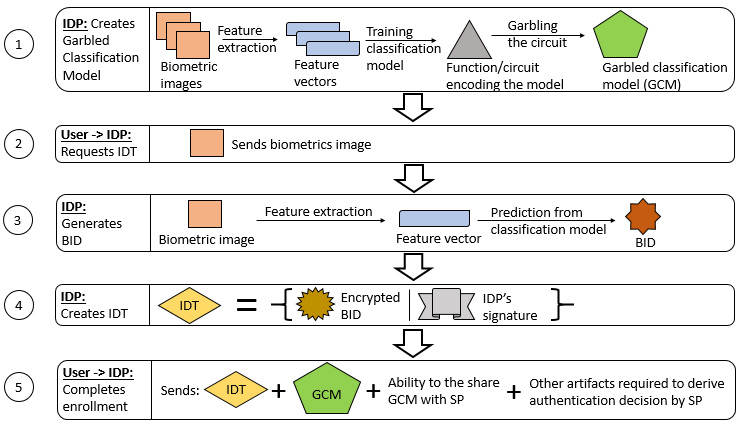
\includegraphics[height=3.00in,width=5.00in]{enrollment}
\caption{Proposed Enrollment Phase}
\label{example}
\end{figure}

\begin{figure}[H]
\centering
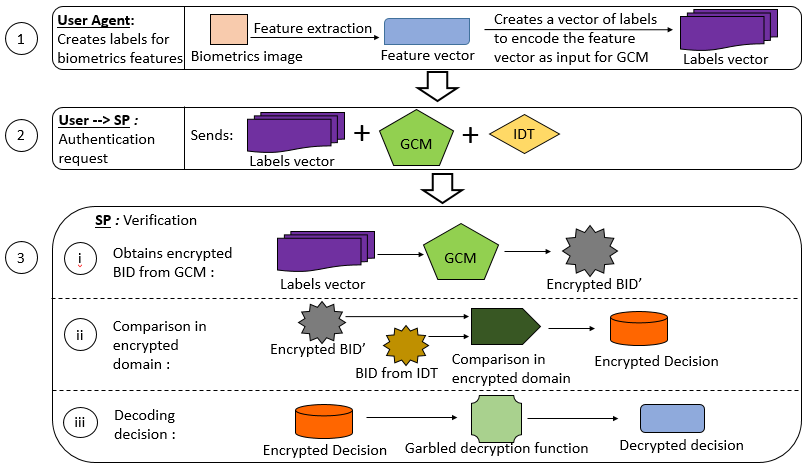
\includegraphics[height=3.00in,width=5.00in]{authentication}
\caption{Proposed Authentication Phase}
\label{example}
\end{figure}

\pagebreak
\subsubsection*{Contribution of this work:}
We aim to produce the following research output:
\begin{enumerate}
 \item Designing a secure and privacy preserving biometrics based remote authentication protocol with aforementioned characteristics, using re-usable 
garbled circuit construct. 
 \item A prototype implementation of the protocol that is able to run in mobile devices.
 \item Security and performance analysis of the protocol.
\end{enumerate}

\footnotesize
\bibliographystyle{IEEEtran}
\bibliography{IEEEabrv,IEEEexample}
 
\end{document}
